\documentclass{beamer}

\usepackage[T1]{fontenc}
\usepackage[latin1]{inputenc}
\usepackage{lmodern}
\usepackage{amsmath,amssymb,amsthm}
\usepackage{graphicx}
\usepackage{tcolorbox}
\usepackage{listings}

\usetheme[headline=section, footlineleft=empty, footlinecenter=empty, footlineright=frames]{TUMCD}
\usefonttheme{professionalfonts}

\lstset{frame=tb, language=Java, aboveskip=3mm, belowskip=3mm, showstringspaces=false, columns=flexible, basicstyle={\small\ttfamily}, numbers=none, numberstyle=\tiny\color{gray}, keywordstyle=\color{blue}, commentstyle=\color{dkgreen}, stringstyle=\color{mauve}, breaklines=true, breakatwhitespace=true, tabsize=3}

\begin{document}

\section{Black Box Model}

\begin{frame}
	\frametitle{Trajectories}
	
	\textbf{Input}
	\begin{itemize}
		\item{Joystick commands: \lstinline{cmd_hst_pt, cmd_crd_pt}}
	\end{itemize}
	
	\vspace{0.5cm}
	
	\textbf{Output}
	\begin{itemize}
		\item{Torques: \lstinline{u_hst, u_crd}}
		\item{Positions: \lstinline{y_hst, y_crd}}
	\end{itemize}

	\vspace{0.5cm}

	Currently we have:
	\begin{itemize}
		\item{\lstinline{n_tra} different trajectories of size \lstinline{n_sim}}
		\item{\lstinline{n_tra = 9; n_sim = 1000}}
		\item{each of them is a matrix of size \lstinline{(n_sim, n_tra)}}	
	\end{itemize}
\end{frame}

\begin{frame}
	\frametitle{Objective Function}
	Parameters that are optimized: \\
	\lstinline{hst_inertia_engine, inertia_yy, hst_friction, crd_mass}
	
	\begin{align*}
		\min_{p\in\mathbb{R}^4} f(p)& = & & \frac{1}{n_{\operatorname{tra}}}
		\cdot\left(\alpha_1\cdot \Vert \overline{U}_{\operatorname{hst}} - U_{\operatorname{hst}}\left(p\right) \Vert_{\operatorname{F}}^2 + \dots \right) \\
		\operatorname{s.t.} & & & p_i \geq 0
	\end{align*}
	
	where
	\begin{align*}
		\alpha_1 & = \frac{1}{\Vert\overline{U}_{\operatorname{hst}}\Vert_{\operatorname{F}}^2} &
		\Vert\overline{U}_{i,j}\Vert_{\operatorname{F}}^2 & = \sum_{j=1}^{n_{\operatorname{tra}}}\sum_{i=1}^{n_{\operatorname{sim}}}|\overline{U}_{i,j}|^2
	\end{align*}
	$\Vert\cdot\Vert_{\operatorname{F}}$ is the Frobenius norm
\end{frame}

\begin{frame}
	\frametitle{Influence of the Parameters}
	$10\%$ deviation of parameter \dots cause in the objective function:
	\begin{itemize}
		\item{\makebox[4cm][l]{\lstinline{hst_inertia_engine}} \makebox[2cm][r]{$1\cdot 10^{-3}$}    \makebox[1cm]{}linear}
		\item{\makebox[4cm][l]{\lstinline{inertia_yy}}         \makebox[2cm][r]{$3.3\cdot 10^{-3}$}  \makebox[1cm]{}linear}
		\item{\makebox[4cm][l]{\lstinline{hst_friction}}       \makebox[2cm][r]{$7.8\cdot 10^{-11}$} \makebox[1cm]{}quadratic}
		\item{\makebox[4cm][l]{\lstinline{crd_mass}}           \makebox[2cm][r]{$52\cdot 10^{-3}$}   \makebox[1cm]{}linear}
	\end{itemize}
	
	\begin{columns}[t]
		\column{.25\linewidth}
			\begin{figure}
				\centering
				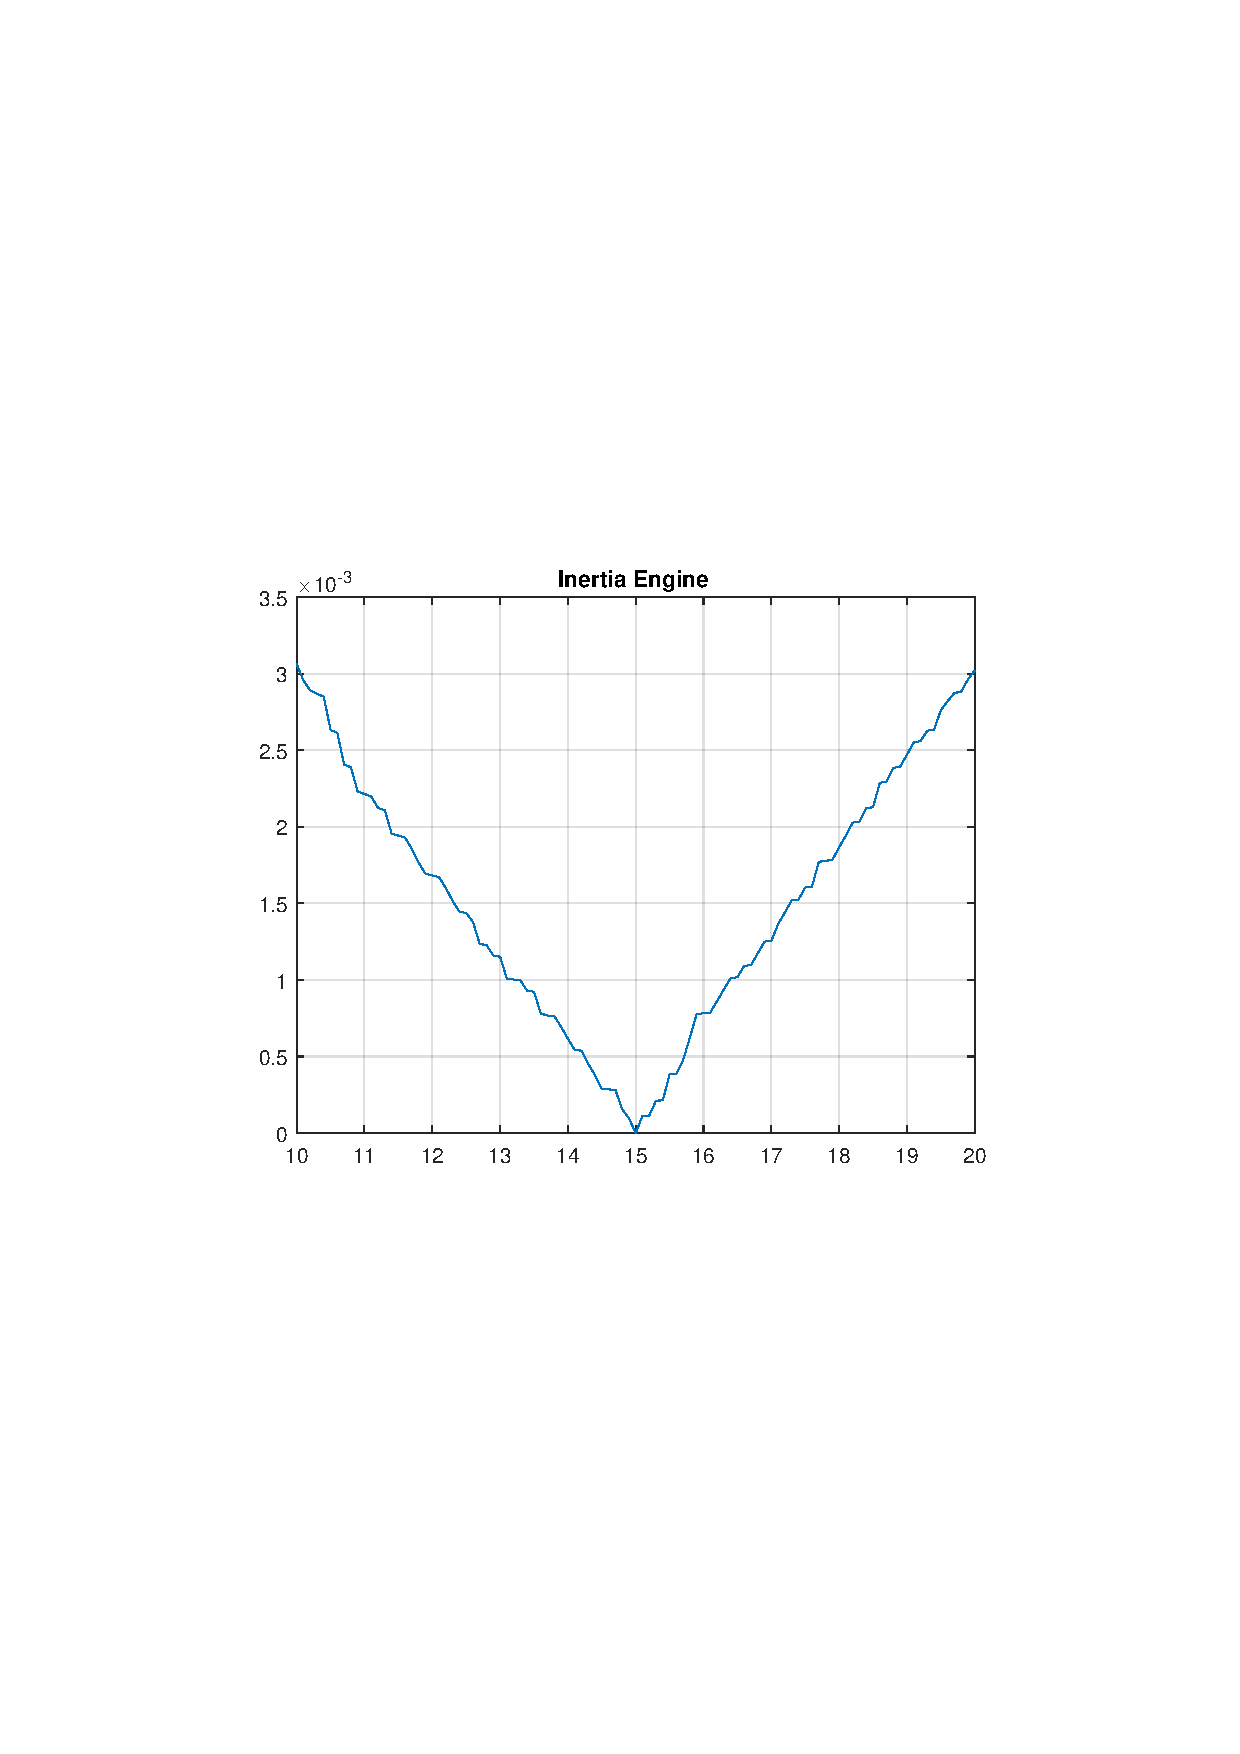
\includegraphics[trim=4cm 9cm 4cm 9cm, clip=true, width=\linewidth]{img/inertia_engine}
			\end{figure}
		\column{.25\linewidth}
			\begin{figure}
				\centering
				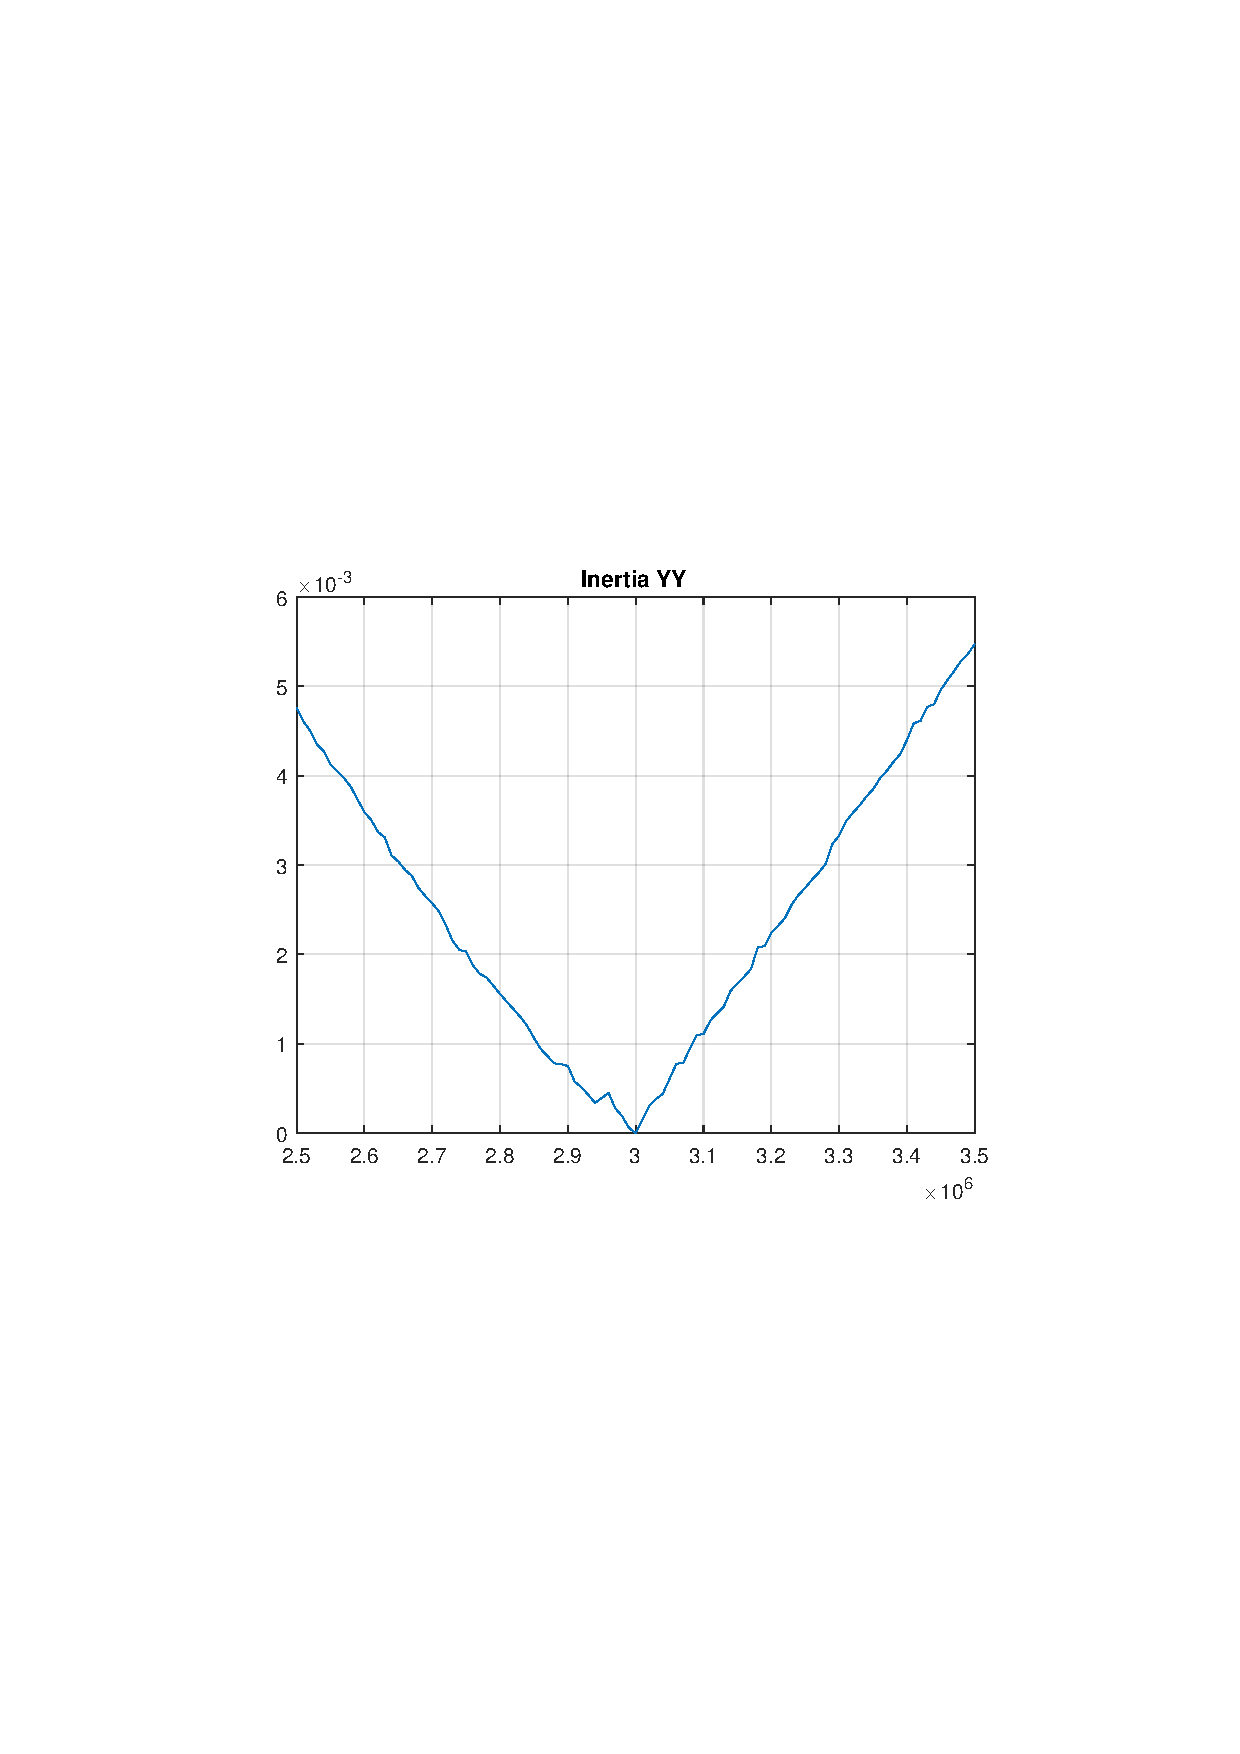
\includegraphics[trim=4cm 9cm 4cm 9cm, clip=true, width=\linewidth]{img/inertia_yy}
			\end{figure}
		\column{.25\linewidth}
			\begin{figure}
				\centering
				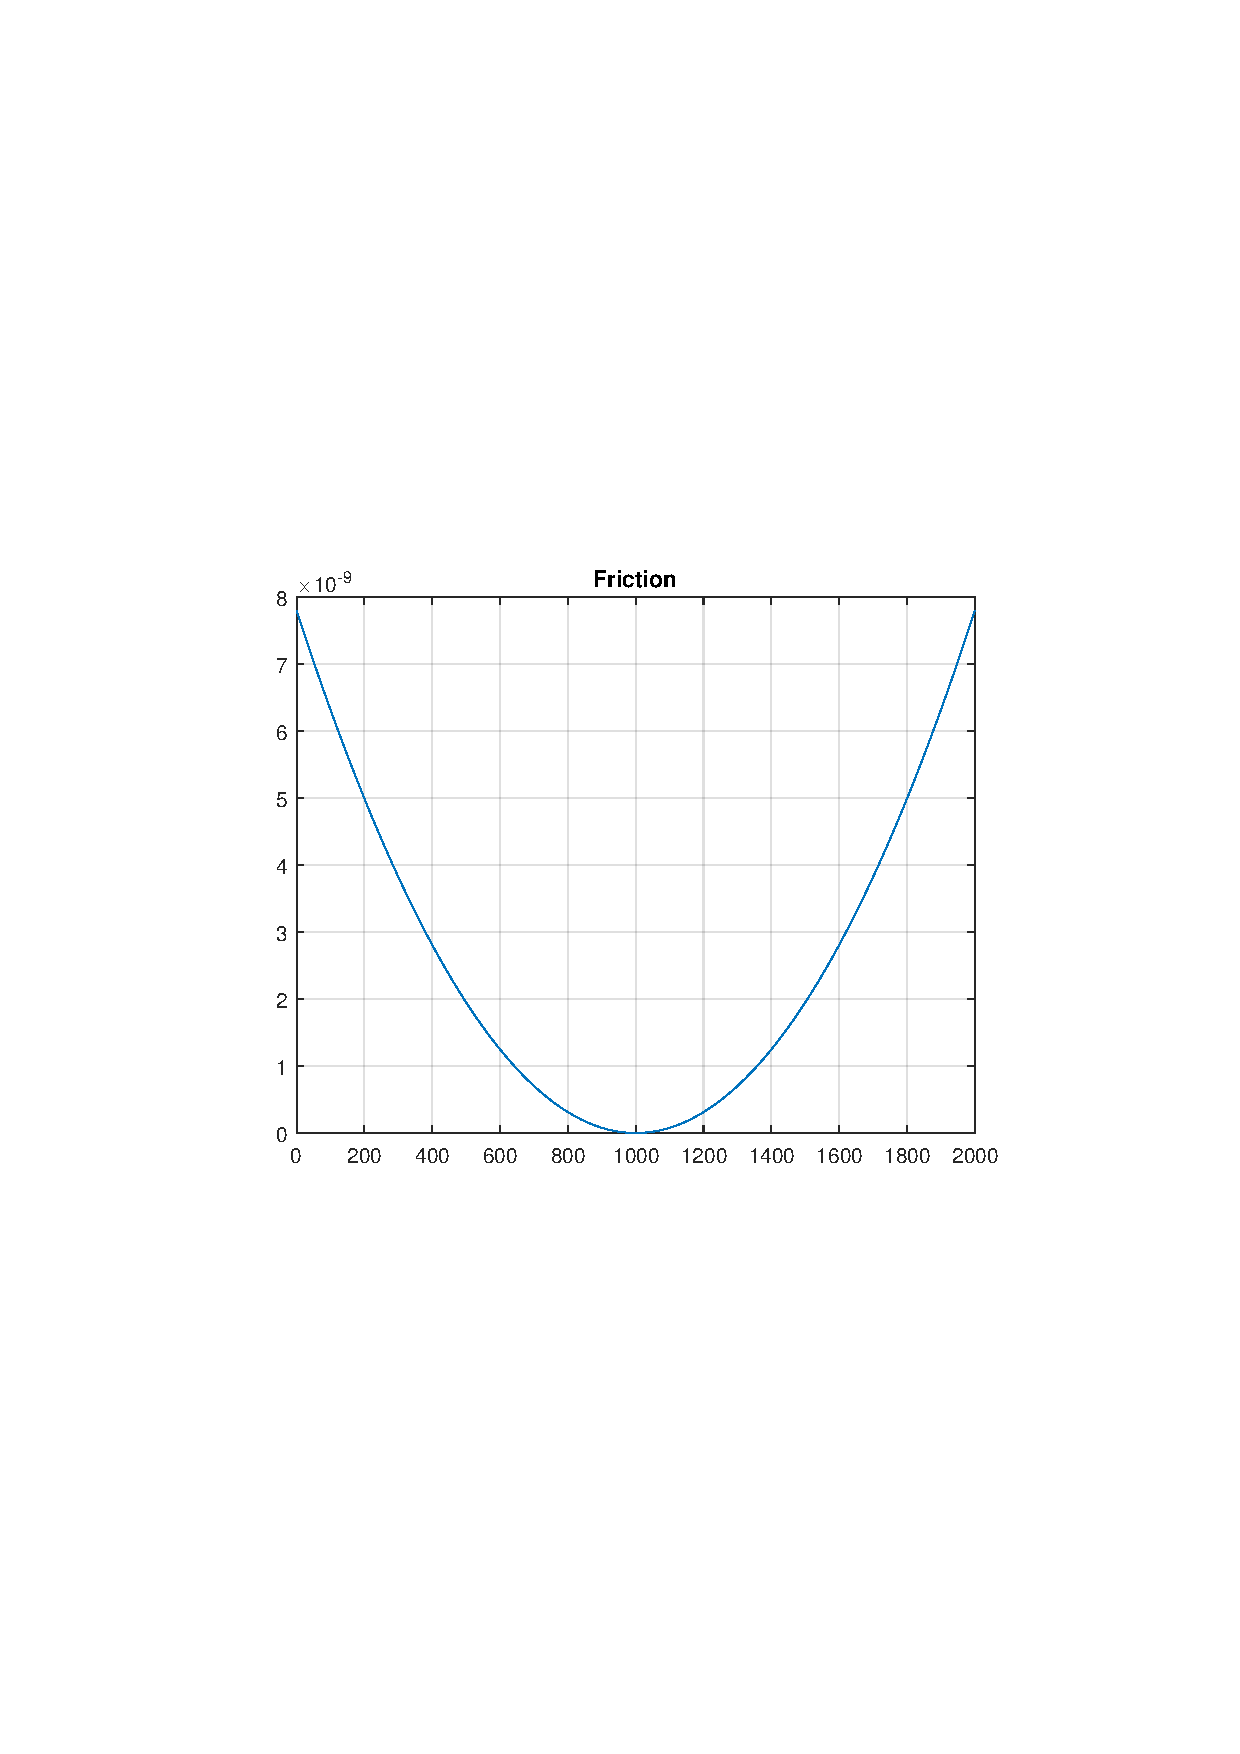
\includegraphics[trim=4cm 9cm 4cm 9cm, clip=true, width=\linewidth]{img/friction}
			\end{figure}
		\column{.25\linewidth}
			\begin{figure}
				\centering
				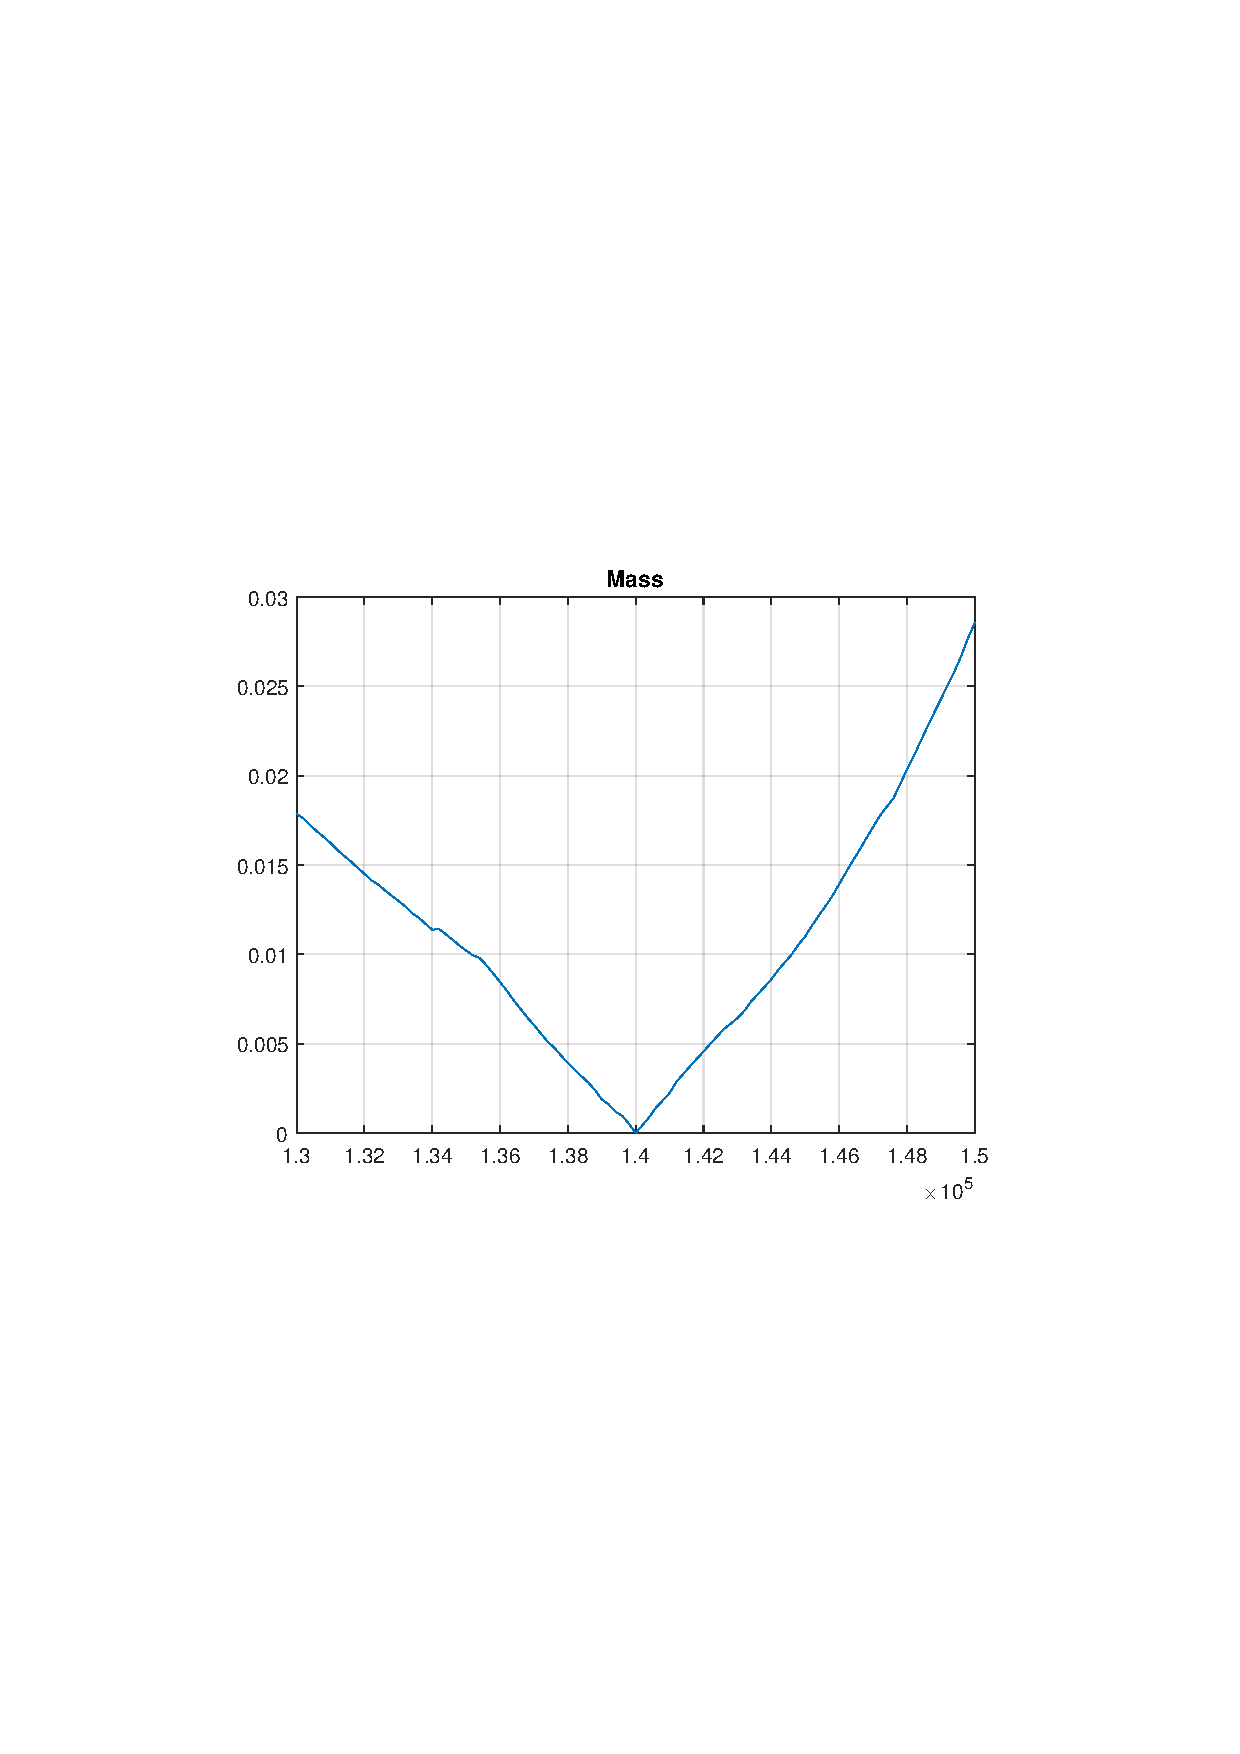
\includegraphics[trim=4cm 9cm 4cm 9cm, clip=true, width=\linewidth]{img/mass}
			\end{figure}
		\end{columns}
\end{frame}

\begin{frame}
	\frametitle{Solvers}
	Conditions:
	\begin{itemize}
		\item{Starting values: $X\sim \operatorname{N}\left(\bar{x},\bar{x}/2\right)$, where $\bar{x}$ is the given value}
		\item{Smarm Size: $10$}
		\item{Function Tolerance: $10^{-9}$}
		\item{Time Limit: 15 min}
		\item{Max Iterations: $\infty$}
	\end{itemize}
	
	 \vspace{0.5cm}
	
	\begin{tabular}{l|ccl}
		& penalty & evaluations & time \\
		\hline
		Particle Swarm & $10^{-13}$ & $2500$ & 3 min \\
		Pattern Search & $10^{-3}$ & $6000$ & 8 min \\
		Genetic Algorithm & $10^{-2}$ & $7500$ & 10 min (time limit) \\
		Simulated Annealing & $10^{-1}$ & $3000$ & 4 min \\
	\end{tabular}
\end{frame}

\end{document}